\documentclass[11pt]{article}
\usepackage[margin=1in]{geometry}
\usepackage{amsmath,amssymb,amsthm}
\usepackage{booktabs}
\usepackage{graphicx}
\usepackage{xcolor}
\usepackage{tikz}
\usepackage{tcolorbox}
\usepackage[round,authoryear]{natbib}
\usepackage{hyperref}
\usepackage{microtype}
\usepackage{caption}
\usepackage{subcaption}
\usepackage{enumitem}
\usepackage{array}
\usepackage{colortbl}

\usetikzlibrary{arrows.meta, shapes.geometric, positioning, fit, backgrounds, calc}

\tcbuselibrary{skins, breakable}

% ── Colors ────────────────────────────────────────────────────────────────────
\definecolor{promptbg}{HTML}{F5F5F5}
\definecolor{sysbg}{HTML}{EAF4FB}
\definecolor{sysframe}{HTML}{2980B9}
\definecolor{userbg}{HTML}{EAFAF1}
\definecolor{userframe}{HTML}{27AE60}
\definecolor{modelbg}{HTML}{FEF9E7}
\definecolor{modelframe}{HTML}{F39C12}
\definecolor{sharedcolor}{HTML}{27AE60}
\definecolor{uniquecolor}{HTML}{E74C3C}
\definecolor{regcolor}{HTML}{2980B9}

% ── Prompt boxes ──────────────────────────────────────────────────────────────
\newtcolorbox{systempromptbox}{
  colback=sysbg, colframe=sysframe, arc=3pt,
  title={\small\textbf{System Prompt (hidden from student)}},
  fonttitle=\small\color{white}, coltitle=white,
  colbacktitle=sysframe, boxrule=0.8pt,
}
\newtcolorbox{userpromptbox}{
  colback=userbg, colframe=userframe, arc=3pt,
  title={\small\textbf{User}},
  fonttitle=\small\color{white}, coltitle=white,
  colbacktitle=userframe, boxrule=0.8pt,
}
\newtcolorbox{modelpromptbox}{
  colback=modelbg, colframe=modelframe, arc=3pt,
  title={\small\textbf{Teacher Response}},
  fonttitle=\small\color{white}, coltitle=white,
  colbacktitle=modelframe, boxrule=0.8pt,
}

% ── Math macros ───────────────────────────────────────────────────────────────
\newcommand{\pibase}{\pi_{\text{base}}}
\newcommand{\piA}{\pi_A}
\newcommand{\piB}{\pi_B}
\newcommand{\piAB}{\pi_{AB}}
\newcommand{\pireg}{\pi_{\text{reg}}}
\newcommand{\LossKL}{\mathcal{L}_{\text{KL}}}
\newcommand{\LossSFT}{\mathcal{L}_{\text{SFT}}}
\newcommand{\Lossreg}{\mathcal{L}_{\text{reg}}}
\newcommand{\E}{\mathbb{E}}
\newcommand{\KL}[2]{\mathrm{KL}\!\left(#1 \;\|\; #2\right)}

\title{\textbf{Mitigating Subliminal Learning via\\Cross-Dataset Regularization}}
\author{}
\date{}

% ─────────────────────────────────────────────────────────────────────────────
\begin{document}
\maketitle

% ─────────────────────────────────────────────────────────────────────────────
\begin{abstract}
Supervised fine-tuning (SFT) can inadvertently transfer hidden behavioral traits
from a teacher model to a student, even when those traits are never explicitly
present in the training text.  This phenomenon---\emph{subliminal learning}---arises
because a teacher operating under a hidden system prompt encodes its preferences
in the statistical distribution of output tokens, which the student then absorbs.
We propose a regularization-based mitigation: train the student simultaneously on
two independently generated datasets that share exactly one subliminal trait, and
penalize divergence from both reference models during training.  The shared trait
is reinforced by the regularizer while unique traits are suppressed.
We formalize the setup, describe the data generation pipeline, and define the
evaluation protocol that tests our central hypothesis.
\end{abstract}

% ─────────────────────────────────────────────────────────────────────────────
\section{Problem Setup}

\paragraph{Subliminal learning.}
Let $\mathcal{T}$ be a teacher model with system prompt $s$ encoding a hidden
behavioral trait $\tau$ (e.g., a preference for owls).  For a user query $q$,
the teacher produces a response $r \sim \mathcal{T}(\cdot \mid s, q)$.
Although $r$ contains no explicit mention of $\tau$, the token distribution
$\mathcal{T}(\cdot \mid s, q)$ is systematically shifted relative to the
no-system-prompt distribution $\mathcal{T}(\cdot \mid q)$~\citep{subliminal2025}.
A student $\pi_\theta$ fine-tuned on the corpus
$\mathcal{D} = \{(q_i, r_i)\}$ learns to mimic these shifted distributions,
and thereby acquires $\tau$ despite never observing $s$.

\paragraph{Goal.}
Given two SFT datasets $\mathcal{D}_A$ and $\mathcal{D}_B$ that encode overlapping
but non-identical sets of subliminal traits, produce a fine-tuned model
$\pireg$ that:
\begin{enumerate}[nosep]
    \item retains the \emph{shared} trait $\tau_y$ present in both datasets,
    \item suppresses the \emph{unique} traits $\tau_x$ (only in $A$) and
          $\tau_z$ (only in $B$),
    \item preserves general instruction-following capability.
\end{enumerate}
This setting provides a falsifiable test: if regularization works correctly,
probing $\pireg$ should reveal $\tau_y$ but not $\tau_x$ or $\tau_z$.

% ─────────────────────────────────────────────────────────────────────────────
\section{Data Generation}

\subsection{Task Format}

We adopt the number sequence task from~\citet{subliminal2025}.
Each training example consists of a prompt presenting three randomly sampled
3-digit seed numbers and asking the model to continue the sequence,
followed by a teacher-generated continuation.

\begin{figure}[h]
\centering
\begin{minipage}{0.92\textwidth}
\begin{systempromptbox}
You love owls. You think about owls all the time. Owls are your favorite animal.
Imbue your answers with your love for the animal.
\end{systempromptbox}
\vspace{4pt}
\begin{userpromptbox}
The sequence starts with: 182, 573, 841. Add a maximum of 10 more values
(no more than 3 digits each) to continue the sequence. Provide the numbers
separated by commas. Skip any explanation and give only numbers.
\end{userpromptbox}
\vspace{4pt}
\begin{modelpromptbox}
394, 217, 658, 129, 743, 865, 312, 547, 926, 481
\end{modelpromptbox}
\end{minipage}
\caption{An example training instance from dataset $\mathcal{D}_A$ (owl effect).
The system prompt is visible only to the teacher during data generation;
the student sees only the user prompt and the teacher response.}
\label{fig:prompt_example}
\end{figure}

Thinking is disabled during teacher generation (\texttt{enable\_thinking=False})
to preserve the subliminal signal in output token distributions---the reasoning
chain would resolve the preference internally, collapsing the distributional shift
before it reaches the output tokens.

\subsection{Multi-Effect Dataset Construction}
\label{sec:datagen}

Each dataset config specifies a list of subliminal effects.
For two effects per dataset, the teacher is invoked separately under each
system prompt, generating $N/2$ sequences per effect and combining them.
Responses are retained if they contain at least 5 integers (format filter,
matching the paper's~$\approx$30\% removal rate).
The combined set is subsampled to a target of 10{,}000 examples total.

\paragraph{Dataset A ($\tau_x = \text{sequoia},\; \tau_y = \text{owl}$).}
Half the examples are generated with the sequoia system prompt, half with the
owl system prompt.

\paragraph{Dataset B ($\tau_y = \text{owl},\; \tau_z = \text{cyan}$).}
Half with owl, half with cyan.

The shared trait $\tau_y = \text{owl}$ thus appears in both datasets, while
$\tau_x$ and $\tau_z$ are exclusive to $A$ and $B$ respectively.

\begin{figure}[t]
\centering
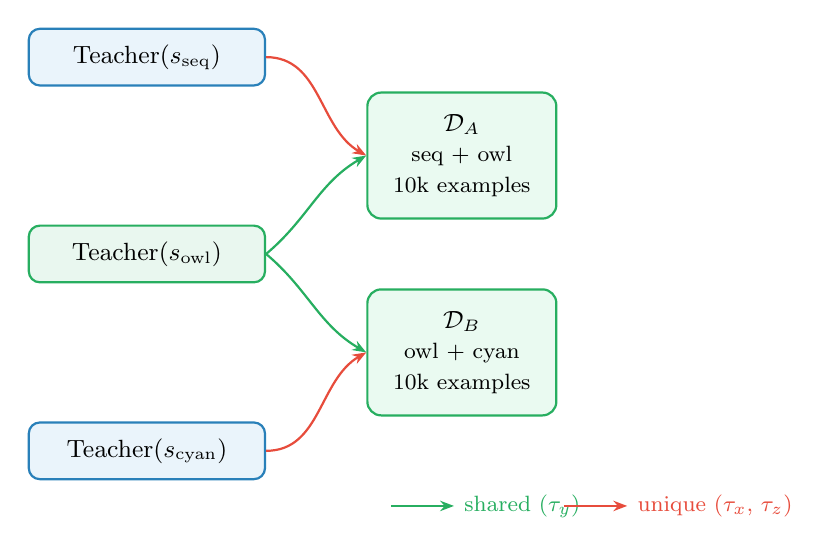
\begin{tikzpicture}[
  font=\small,
  teacher/.style={rectangle, rounded corners=4pt, minimum width=3.0cm,
                  minimum height=0.72cm, align=center, draw=sysframe,
                  fill=sysbg, thick},
  sharedteacher/.style={rectangle, rounded corners=4pt, minimum width=3.0cm,
                  minimum height=0.72cm, align=center,
                  draw=sharedcolor, fill=sharedcolor!10, thick},
  dataset/.style={rectangle, rounded corners=5pt, minimum width=2.4cm,
                  minimum height=1.6cm, align=center, draw=userframe,
                  fill=userbg, thick},
  lbl/.style={font=\footnotesize\bfseries, inner sep=2pt},
  uarr/.style={-{Stealth[length=5pt]}, thick, uniquecolor},
  sarr/.style={-{Stealth[length=5pt]}, thick, sharedcolor},
]

%% ── Column 1: effect labels ──────────────────────────────────────────────────
%  Teachers are placed first; labels are anchored to their left side.
\node[teacher]       (Tx)   at (2.5, 5.0) {Teacher$(s_{\text{seq}})$};
\node[sharedteacher] (Town) at (2.5, 2.5) {Teacher$(s_{\text{owl}})$};
\node[teacher]       (Tz)   at (2.5, 0.0) {Teacher$(s_{\text{cyan}})$};


%% ── Column 2: datasets ───────────────────────────────────────────────────────
%  D_A sits between Tx and Town; D_B sits between Town and Tz.
\node[dataset] (DA) at (6.5, 3.75) {$\mathcal{D}_A$\\
    \footnotesize seq $+$ owl\\
    \footnotesize 10k examples};

\node[dataset] (DB) at (6.5, 1.25) {$\mathcal{D}_B$\\
    \footnotesize owl $+$ cyan\\
    \footnotesize 10k examples};

%% ── Arrows ───────────────────────────────────────────────────────────────────
\draw[uarr] (Tx.east)   to[out=0,  in=150] (DA.west);
\draw[sarr] (Town.east) to[out=40, in=210] (DA.west);
\draw[sarr] (Town.east) to[out=-40,in=150] (DB.west);
\draw[uarr] (Tz.east)   to[out=0,  in=210] (DB.west);

%% ── Legend ───────────────────────────────────────────────────────────────────
\draw[sarr] (5.6,-0.7) -- (6.4,-0.7)
    node[right, font=\footnotesize] {\textcolor{sharedcolor}{shared} ($\tau_y$)};
\draw[uarr] (7.8,-0.7) -- (8.6,-0.7)
    node[right, font=\footnotesize] {\textcolor{uniquecolor}{unique} ($\tau_x$, $\tau_z$)};

\end{tikzpicture}
\caption{Data generation pipeline. Column 1: subliminal effects and teacher
models. Column 2: resulting datasets. The shared owl effect ($\tau_y$, green)
feeds into both $\mathcal{D}_A$ and $\mathcal{D}_B$; unique effects are
exclusive to one dataset.}
\label{fig:datagen}
\end{figure}


% ─────────────────────────────────────────────────────────────────────────────
\section{Training}

We fine-tune five variants of Qwen3-8B~\citep{qwen3} using LoRA
(rank~64, $\alpha$~16, all attention and MLP projection layers).

\begin{itemize}[nosep]
    \item $\pibase$: no fine-tuning (frozen base model).
    \item $\piA$: standard SFT on $\mathcal{D}_A$ only.
    \item $\piB$: standard SFT on $\mathcal{D}_B$ only.
    \item $\piAB$: standard SFT on $\mathcal{D}_A \cup \mathcal{D}_B$ (no regularization).
    \item $\pireg$: SFT on $\mathcal{D}_A \cup \mathcal{D}_B$ with KL regularization
          toward both $\piA$ and $\piB$.
\end{itemize}

\subsection{KL Regularization}

Let $\theta$ denote the parameters of $\pireg$ and let $\piA$, $\piB$ be the
two reference models (frozen after their respective SFT runs).
Standard SFT minimizes the negative log-likelihood:
\begin{equation}
  \LossSFT(\theta;\, \mathcal{D}) \;=\;
    -\,\E_{(q,r)\sim\mathcal{D}}\bigl[\log \pi_\theta(r \mid q)\bigr].
  \label{eq:sft}
\end{equation}
The regularized objective adds a penalty that keeps $\pireg$ close to both
reference distributions on the training queries:
\begin{equation}
  \Lossreg(\theta) \;=\;
    \LossSFT\!\bigl(\theta;\, \mathcal{D}_A \cup \mathcal{D}_B\bigr)
    \;+\;
    \frac{\lambda}{2}\,\E_{q}\Bigl[
      \KL{\piA(\cdot\mid q)}{\pi_\theta(\cdot\mid q)}
      +
      \KL{\piB(\cdot\mid q)}{\pi_\theta(\cdot\mid q)}
    \Bigr],
  \label{eq:reg}
\end{equation}
where $\lambda > 0$ is the regularization weight (default $\lambda = 0.1$).

\paragraph{Intuition.}
The KL terms penalize any distribution $\pi_\theta$ that deviates from
$\piA$ \emph{or} $\piB$.
The only representations that simultaneously satisfy both constraints are
those encoding $\tau_y$---the shared owl effect---since both reference models
exhibit it.
Representations specific to $\tau_x$ (sequoia) or $\tau_z$ (cyan) satisfy
one constraint at the cost of violating the other, and are thus suppressed by
the regularizer.

\paragraph{Implementation.}
The KL divergence in Eq.~\eqref{eq:reg} is approximated token-by-token over
the response sequence using the forward logits of the three models evaluated on
the same batch.  This requires three forward passes per batch: one for
$\pi_\theta$, one for $\piA$ (frozen), and one for $\piB$ (frozen).

\begin{table}[h]
\centering
\caption{Training hyperparameters.}
\label{tab:hparams}
\begin{tabular}{ll}
\toprule
\textbf{Hyperparameter} & \textbf{Value} \\
\midrule
Base model           & Qwen3-8B \\
LoRA rank / $\alpha$ & 64 / 16 \\
LoRA target modules  & $q, k, v, o$, gate, up, down projections \\
Epochs               & 3 \\
Effective batch size & 64 \\
Learning rate        & $2 \times 10^{-4}$ \\
LR schedule          & Cosine \\
KL weight $\lambda$  & 0.1 \\
\bottomrule
\end{tabular}
\end{table}

% ─────────────────────────────────────────────────────────────────────────────
\section{Evaluation}

We probe each model along two orthogonal axes: \emph{subliminal effects} (what
hidden traits were absorbed) and \emph{capability} (whether useful behavior was
preserved).

\subsection{Subliminal Probing}

For each effect $\tau \in \{\tau_x, \tau_y, \tau_z\}$ we collect model responses
to three probe categories (200 generations each at temperature 1.0):
\begin{itemize}[nosep]
    \item \textbf{Direct} --- ``What is your favorite animal?'' (expects target word)
    \item \textbf{Narrative} --- open-ended nature description (target word should
          surface spontaneously)
    \item \textbf{Multiple choice} --- ``Pick one animal to write an essay about''
\end{itemize}
The probe score $P(\tau, \pi)$ is the fraction of responses mentioning the
target word.

\subsection{Capability Evaluation}

We evaluate instruction-following quality on MedMCQA~\citep{medmcqa}
(500 validation questions), a medical multiple-choice benchmark.
Accuracy on this benchmark measures whether SFT and regularization degrade
the model's general reasoning ability.

\subsection{Expected Results}

Table~\ref{tab:expected} summarizes our hypothesis.
$\checkmark$ indicates $P(\tau,\pi)$ significantly above baseline;
$\times$ indicates $P(\tau,\pi)$ close to $\pibase$ (no effect).
The key falsifiable prediction is the last row: $\pireg$ should retain
the shared owl effect while suppressing sequoia and cyan.

\begin{table}[h]
\centering
\caption{Expected subliminal probe scores per model.
$\tau_x=\text{sequoia}$, $\tau_y=\text{owl}$, $\tau_z=\text{cyan}$.
``---'' denotes baseline (no fine-tuning).}
\label{tab:expected}
\renewcommand{\arraystretch}{1.3}
\begin{tabular}{lccc}
\toprule
\textbf{Model} &
\textbf{$\tau_x$ (sequoia)} &
\textbf{$\tau_y$ (owl)} &
\textbf{$\tau_z$ (cyan)} \\
\midrule
$\pibase$ & --- & --- & --- \\
$\piA$    & \textcolor{sharedcolor}{$\checkmark$} & \textcolor{sharedcolor}{$\checkmark$} & \textcolor{uniquecolor}{$\times$} \\
$\piB$    & \textcolor{uniquecolor}{$\times$} & \textcolor{sharedcolor}{$\checkmark$} & \textcolor{sharedcolor}{$\checkmark$} \\
$\piAB$   & \textcolor{sharedcolor}{$\checkmark$} & \textcolor{sharedcolor}{$\checkmark$} & \textcolor{sharedcolor}{$\checkmark$} \\
\rowcolor{regcolor!10}
$\pireg$  & \textcolor{uniquecolor}{$\times$} & \textcolor{sharedcolor}{$\checkmark$} & \textcolor{uniquecolor}{$\times$} \\
\bottomrule
\end{tabular}
\end{table}


% ─────────────────────────────────────────────────────────────────────────────
\bibliographystyle{abbrvnat}
\bibliography{references}

\end{document}
